Under the condition of \textbeta-stable, the proton's contribution $x_p = n_p/n_b$ to the baryon density of of neutrino-free \gls{NS} matter is given by Figure \ref{fig:xp}, computed with 5 different versions of the density-dependent \gls{NN} interaction. It can be seen that in all cases, the higher the density, the more protons there are in the baryon composition. Furthermore, with the newly introduced parameterization of spin-dependent terms (10 and 11) in all 6 interactions, generally the protons are more abundant at higher polarization, which can be seen with the height of each ``bump'' in Figure \ref{fig:xp} at low density, while the highes mass possible \gls{NS} for each configuration tends to decrease with increasing incompressibility $K$, i.e. different model.
\begin{figure}[ht!]
        \centering
        \includegraphics[width=\textwidth]{fig/xp.eps}
        \caption{Proton fraction $x_p$ of \textbeta-stable \gls{NM} at different baryon density and spin polarization for different density-dependent \gls{NN} interactions. The lower horizontal lines are the \gls{DU} threshold \eqref{eq:xDU} and the dot at the end of each line corresponds to the highest mass \gls{NS}'s central density of each model. The two rows of figures correspond to two previously defined scenarios, i.e. A and B.}
        \label{fig:xp}
\end{figure} 
The density-dependent proton fraction $x_p$ is also an essential input for determining the cooling rate of the \gls{NS}, in which the dominant direct Urca (\gls{DU}) process of \gls{NS} cooling by $\nu$ emission \citep{lattimer2004physics}, i.e.
\begin{equation}
    n \longrightarrow p + e^- +\bar{\nu}_e \quad\text{and}\quad p \longrightarrow n + e^+ + \nu_e,
\end{equation}
can only take place if the proton fraction exceeds the threshold \citep{loan2011equation}
\begin{equation}
    x_{DU} = \frac{1}{ 1 + \left[ 1 + \left( \frac{n_e}{n_e + n_\mu} \right)^{1/3} \right]^3 }
    \label{eq:xDU}
\end{equation}
Note that the thresholds $x_{DU}$ determined in these calculations remain fairly unchanged in the whole range of baryon density, as well as when the polarization varies or at different models, which can be explained by the absence of interaction between leptons and baryons in the current study. The threshold also ranges from $\approx 11\%$ at low density, due to the absence of muon, to $\approx 15\%$ as $n_b$ increases, which is consistent with the range deduced from the study of \cite{lattimer1991direct}. The proton fraction $x_p$ in this case increases significantly as the value of $\Delta_0$ rises to $\approx 1$, however, due to the localization of magnetic field in the surface, all models in the two scenarios commonly surpass the \gls{DU} threshold at a high density of $\lesssim 5n_0$. Beside, the electron fraction infered by this result is around $\gtrsim 10\%$, which is however much lower than the observed quantity $\approx 27\%$ from the blue kilonova ejecta following the GW170817 event \citep{abbott2017gw170817, evans2017swift} and can very possibly come from a magnetar as suggested by \cite{metzger2018magnetar}.\par
\begin{figure}[ht!]
        \centering
        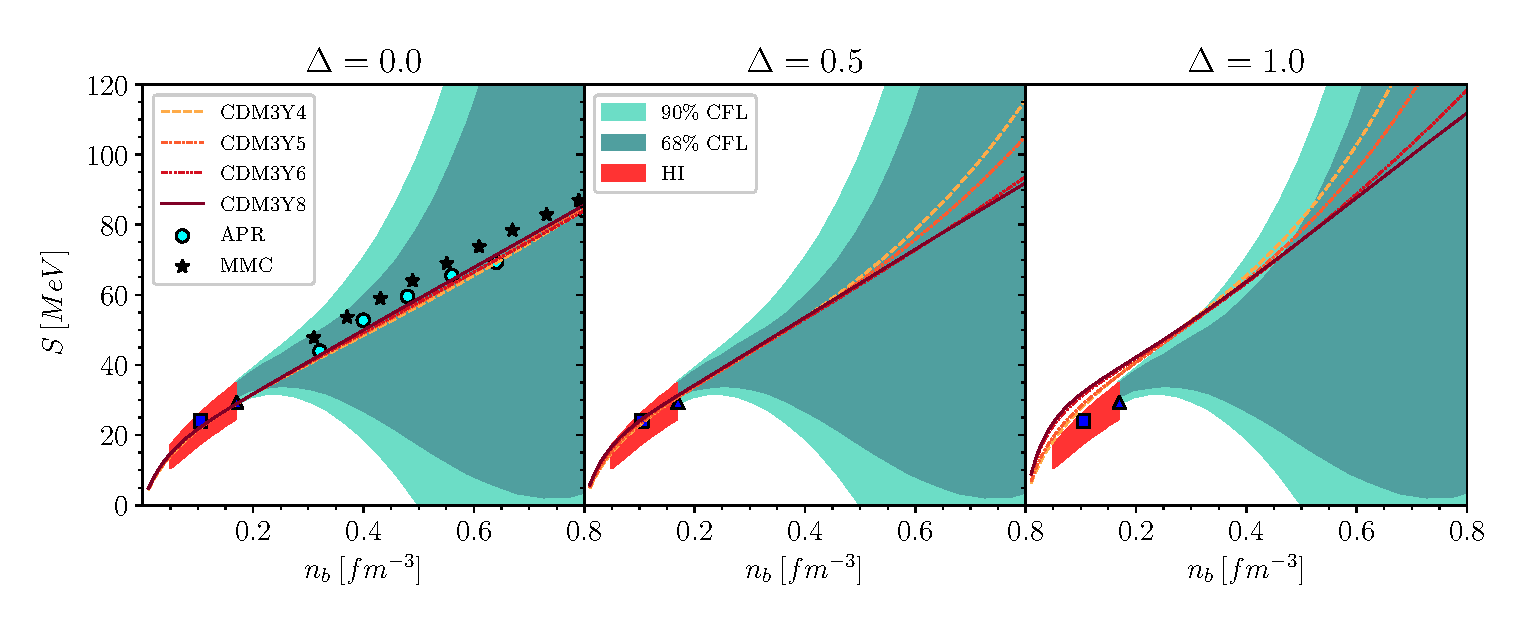
\includegraphics[width=\textwidth]{fig/S.eps}
        \caption{Symmetric energy $S$ of symmetric \gls{NM} at increasing polarization with 5 CDM3Y$n$ interaction models. The shaded areas are the empirical ranges obtained from the Bayesian study \citep{xie2019bayesian} of the \gls{NS} of radius $R_{1.4}$ at 68\% and 90\% confident level (\gls{CFL}) with the GW170817 event \citep{abbott2018gw170817}. The square and triangle are the values suggested by the structure study of \cite{trippa2008giant} and \cite{furnstahl2002neutron}. The circles and stars are the ab-initio result of \cite{akmal1998equation} (\gls{APR}) and microscopic Monte Carlo (\gls{MMC}) calculation by \cite{gandolfi2010microscopic}.}
        \label{fig:s}
\end{figure} 
\begin{figure}[ht!]
    \centering
    \includegraphics[width=\textwidth]{fig/EAS.eps}
    \caption{Same as Figure \ref{fig:s} for the energy per baryon $E/A$ of symmetric \gls{NM}.}
    \label{fig:eas}
\end{figure} 
The nuclear symmetry energy is well constrained at low baryon density by the study of heavy-ion (\gls{HI}) collisions \citep{tsang2011constraints,ono2003isospin}, the structure study of the giant dipole resonance by \cite{trippa2008giant} or the neutron skin \citep{furnstahl2002neutron}. As shown in Figure \ref{fig:s}, the symmetry energy $S$ \eqref{eq:S} of spin saturated ($\Delta = 0$) symmetric ($\delta = 0$) \gls{NM} is calculated for each interaction in each scenario and compared to the empirical data. It's clear that at high baryon density $n_b$, the nuclear symmetry energy doesn't vary much from each others and from scenario to scenario, as well as being well within the astrophysical constraint from GW170817 by \cite{xie2019bayesian}. However, in the low density region, due to the large variation of spin polarization $\Delta$, the calculated $S$ only follow the empirical constraint when the \gls{NS} surface is partially polarized, i.e. the total polarization case $\Delta_0 \approx 1$ is very unlikely to occur.\par
The same conclusion can be drawn from the energy per baryon $E/A$ of symmetric \gls{NM} (Figure \ref{fig:eas}), as it is in good agreement with the empirical data \citep{akmal1998equation,gandolfi2010microscopic} at the spin saturated central region with $n_b \gtrsim 2n_0$ and even at low density if the surface is not endowed in strong magnetic field ($\Delta\approx 0$), similar to the work of \cite{tan2021equation}. The astrophysical constraint from GW170817, on the other hand, is much narrower than that for the nuclear symmetry energy and. Thus for this quantity, the version CDM3Y3 can be ruled out due to it being outside of the 90\% region of the GW170817 constraint while the other versions with higher incompressibility $K$ still remain within. The incompressibility $K$ at saturation density $n_0$ is shown in the Table \ref{tab:pars} for different scenario mentioned.\par
The incompressibility $K$ of symmetric \gls{NM} has been intensively studied in several structure studies of monopole excitations (e.g. \cite{garg2018compression}), \gls{HI} collisions and refractive \gls{NN} scattering \citep{khoa2007nuclear}. The \gls{HF} result in Table \ref{tab:pars} gives a wide range of $K\approx 300-491\: MeV$ for scenario B, which is thus ruled out due to it being outside of the constrained value $K\approx 240^{+20}_{-20}\:MeV$, while scenario A returns a much smaller range of $K\approx 217-271\:MeV$ and agrees well with the constraint. In this scenario, the spin polarization $\Delta$ at saturation density $n_0$ is relatively close to $0$, thus makes the result close to that of \cite{tan2020spin}. Apart from the nuclear incompressibility $K$, the present \gls{HF} calculation gives rise to other quantities, i.e. the symmetry coefficient $J$, the slope parameter $L$ and the curvature parameter $K_{sym}$ \eqref{eq:pars}, whose results are also given in Table \ref{tab:pars}. Recently, the values of $J$, $L$, $K_{sym}$ are much more well determined from the study of \cite{essick2021astrophysical} by combining astrophysical data with PREX-II and chiral effective field theory, which yields $J\approx 34^{+3}_{-3}\:MeV$, $L\approx 58^{+19}_{-19}\:MeV$ and $K_{sym}\approx -107^{+128}_{-138}\:MeV$. The value of $J$ and $L$ obtained with \gls{HF} formalism remain well within the interval suggested by the study of \cite{essick2021astrophysical}, as well as the curvature $K_{sym}$, however, the value of $K_{sym}$ has not been as well determined as the other quantities, therefore it still widely ranges for different scenarios.\par
\begin{table}[ht!]
    \centering
    \caption{The symmetry coefficient $J$, slope parameter $L$, curvature $K_{sym}$ of the symmetric energy \eqref{eq:pars} and incompressibility $K$ \eqref{eq:K} of symmetric \gls{NM}, calculated using 6 different \gls{NN} interactions.}
    \label{tab:pars}
    \begin{tabular}{|c|c|C|C|C|C|C|}
        \hline
        Interaction & Scenario & \Delta_0 & J & L & K_{sym} & K\\
        \hline
        \multirow{6}{*}{CDM3Y3} & \multirow{3}{*}{A} & 0.6 & 28.96 & 48.40 & -68.59 & 217.80\\
        \cline{3-7}
                                & & 0.8 & 28.97 & 48.42 & -68.54 & 218.295\\
        \cline{3-7}
                                & & 1.0 & 28.99 & 48.46 & -68.47 & 218.93\\
        \cline{2-7}
                                & \multirow{3}{*}{B} & 0.6 & 30.90 & 52.94 & -62.81 & 300.90\\
        \cline{3-7}
                                & & 0.8 & 32.46 & 56.09 & -62.46 & 366.29\\
        \cline{3-7}
                                & & 1.0 & 34.56 & 59.83 & -66.58 & 450.94\\
        \hline
        \multirow{6}{*}{CDM3Y4} & \multirow{3}{*}{A} & 0.6 & 28.98 & 48.40 & -60.43 & 228.44\\
        \cline{3-7}
                                & & 0.8 & 28.99 & 48.44 & -60.37 & 228.81\\
        \cline{3-7}
                                & & 1.0 & 29.00 & 48.47 & -60.31 & 229.29\\
        \cline{2-7}
                                & \multirow{3}{*}{B} & 0.6 & 30.73 & 52.43 & -54.70 & 291.17\\
        \cline{3-7}
                                & & 0.8 & 32.16 & 55.27 & -53.59 & 340.53\\
        \cline{3-7}
                                & & 1.0 & 34.09 & 58.72 & -55.90 & 404.45\\
        \hline
        \multirow{6}{*}{CDM3Y5} & \multirow{3}{*}{A} & 0.6 & 28.94 & 48.39 & -49.55 & 241.78\\
        \cline{3-7}
                                & & 0.8 & 28.95 & 48.41 & -49.50 & 242.20\\
        \cline{3-7}
                                & & 1.0 & 28.96 & 48.43 & -49.44 & 242.74\\
        \cline{2-7}
                                & \multirow{3}{*}{B} & 0.6 & 30.68 & 51.27 & -43.81 & 312.46\\
        \cline{3-7}
                                & & 0.8 & 32.11 & 53.29 & -41.68 & 368.07\\
        \cline{3-7}
                                & & 1.0 & 34.04 & 55.73 & -41.68 & 440.09\\
        \hline
        \multirow{6}{*}{CDM3Y6} & \multirow{3}{*}{A} & 0.6 & 28.96 & 48.38 & -42.02 & 252.34\\
        \cline{3-7}
                                & & 0.8 & 28.97 & 48.39 & -41.97 & 252.72\\
        \cline{3-7}
                                & & 1.0 & 28.99 & 48.40 & -41.90 & 253.20\\
        \cline{2-7}
                                & \multirow{3}{*}{B} & 0.6 & 31.08 & 49.86 & -34.22 & 316.04\\
        \cline{3-7}
                                & & 0.8 & 32.77 & 50.67 & -29.57 & 366.17\\
        \cline{3-7}
                                & & 1.0 & 35.03 & 51.41 & -25.62 & 431.11\\
        \hline
        \multirow{6}{*}{CDM3Y8} & \multirow{3}{*}{A} & 0.6 & 28.97 & 48.40 & -28.59 & 257.74\\
        \cline{3-7}
                                & & 0.8 & 28.98 & 48.41 & -28.55 & 258.21\\
        \cline{3-7}
                                & & 1.0 & 29.00 & 48.42 & -28.49 & 258.82\\
        \cline{2-7}
                                & \multirow{3}{*}{B} & 0.6 & 31.22 & 49.54 & -22.16 & 337.89\\
        \cline{3-7}
                                & & 0.8 & 33.01 & 50.04 & -18.40 & 400.98\\
        \cline{3-7}
                                & & 1.0 & 35.40 & 50.35 & -15.43 & 482.68\\
        \hline
        \multirow{6}{*}{BDM3Y1} & \multirow{3}{*}{A} & 0.6 & 28.99 & 48.38 & -11.90 & 270.74\\
        \cline{3-7}
                                & & 0.8 & 29.01 & 48.38 & -11.87 & 271.21\\
        \cline{3-7}
                                & & 1.0 & 29.03 & 48.37 & -11.83 & 271.80\\
        \cline{2-7}
                                & \multirow{3}{*}{B} & 0.6 & 31.47 & 47.03 & -5.40 & 349.49\\
        \cline{3-7}
                                & & 0.8 & 33.43 & 45.63 & 0.72 & 411.48\\
        \cline{3-7}
                                & & 1.0 & 36.01 & 43.47 & 8.88 & 491.78\\
        \hline
    \end{tabular}
\end{table}
In Figure \ref{fig:p}, we show the total pressure of \gls{NS} matter $P(n_b)$ following the \gls{HF} calculation of 6 different versions of the density-dependent \gls{NN} interaction endowed with different scenarios. Unsurprisingly, at low density, the pressure is higher than its supposed value because of the existence of strong magnetic field at the surface. These results are simultaneously compared with the empirical pressure obtained from the ``spectral'' \gls{EoS} inferred from the Bayesian analysis of the GW170817 event. It is clear that the larger $K$ an interaction version has (Table \ref{tab:cd}), the more the generated \gls{NM} can be compressed to higher pressure at high density, and the model CDM3Y3 and CDM3Y4 can be excluded since they would most likely not satisfy the constraint derived by \cite{abbott2018gw170817}, while the other 4 versions still lie inside of the 90\% \gls{CFL} region. In general, the pressures calculated by these 4 models follow well the empirical values from $\approx \rho_0$ to their corresponding maximum central density, i.e. the total pressure at twice and six times nuclear saturation density is within the range $P(2\rho_0)\approx 3.5^{+2.7}_{-1.7}\times 10^{34}$ and $P(6\rho_0)\approx 9.0^{+7.9}_{-2.6}\times 10^{35}\:dyn/cm^2$ at 90\% \gls{CFL}.  Plus, at increasing spin polarization, the pressure tends to be stronger, indicated by a raise of $P(\rho_b)$ at the low density region. Taking all of the \gls{EoS} constraint up until now into account, the value suggested by the empirical study tends to favor models with higher $K$ value and smaller spin polarization.\par
\begin{figure}[ht!]
        \centering
        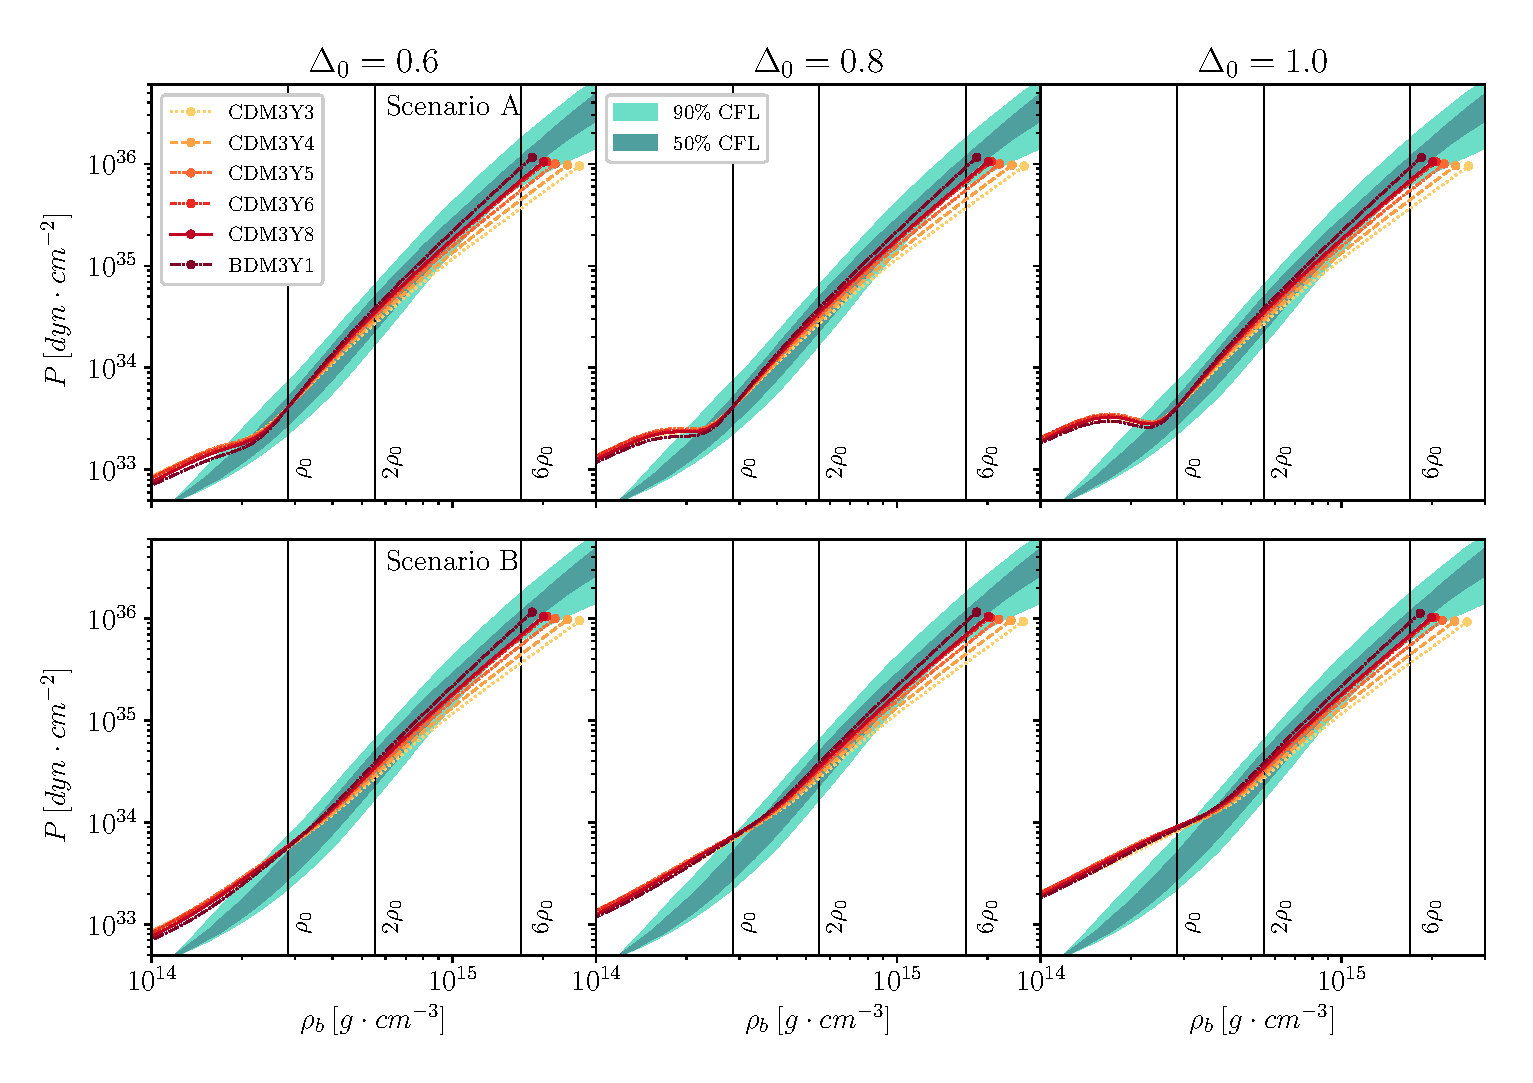
\includegraphics[width=\textwidth]{fig/P.eps}
        \caption{Same as Figure \ref{fig:s} for the pressure $P$ as a function of \emph{rest baryon mass density} $\rho_b$ along with empirical pressure given by the ``Spectral'' \gls{EoS} from the Bayesian analysis of the GW170817 data \citep{abbott2018gw170817} with 50\% (light gray) and 90\% (dark gray) confidence level. The dot at the end of each line corresponds to the central baryon density $n_b$ of maximum \gls{NS} mass.}
        \label{fig:p}
\end{figure} 
\begin{figure}[ht!]
        \centering
        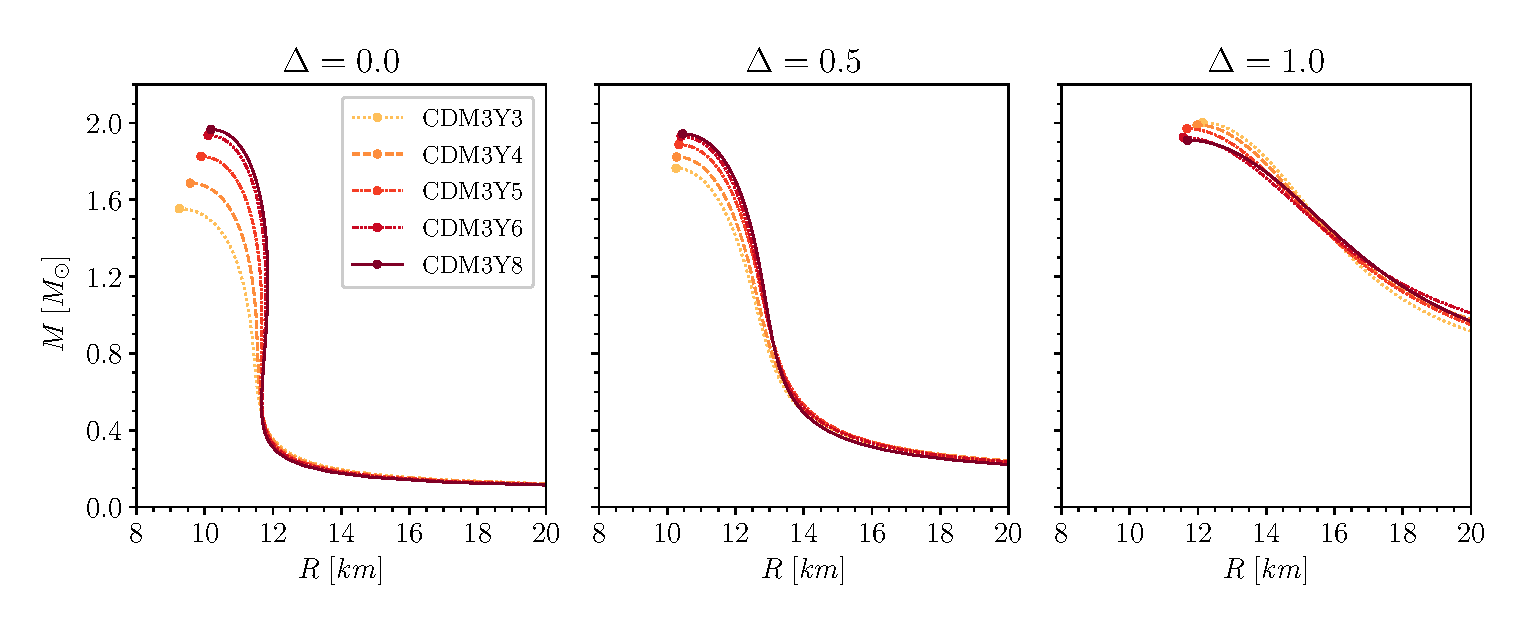
\includegraphics[width=\textwidth]{fig/MR.eps}
        \caption{The relation between gravitational mass $M$ and the radius $R$ of the \gls{NS} according to the corresponding model and polarization. The GW170817 constraint for \gls{NS} with mass $1.4M_\odot$ is shown by the colored contour, where the blue (red) shaded area represents the heavier (lighter) \gls{NS} \citep{abbott2018gw170817}. The dot in each line indicates the maximum \gls{NS} mass of the each model. The dark and light orange region indicates the mass of the second \gls{PSR} J0348+0432 \citep{antoniadis2013massive} and millisecond \gls{PSR} J0740+6620 \citep{cromartie2020relativistic} respectively.}
        \label{fig:mr}
\end{figure} 
With the previously defined \gls{NN} interactions, each model generates a \textbeta-stable $npe\mu$ matter that traces a $M(R)$ relation of the \gls{NS} for every different $\Delta(n_b)$ configuration, which are shown in Figure \ref{fig:mr} in comparison with the GW170817 constraint \citep{abbott2018gw170817}, as well as the lower mass limit of the second \gls{PSR} J0348+0432 ($M\approx 2.01^{+0.04}_{-0.04}M_\odot$) and the millisecond \gls{PSR} J0740+6620 ($M\approx 2.14^{+0.20}_{-0.18}M_\odot$), i.e. the heaviest \glsplural{NS} observed so far. Notably, it is interesting that all 6 versions of the interaction here remain inside the empirical range at $M=1.4M_\odot$ at $\Delta_0 = 0.6$ and the scenario A when $\Delta_0 = 0.8$; the configurations with $\Delta_0 = 1.0$, unsurprisingly, give unsatisfying result, similar to the conclusion reached by \cite{tan2020spin} and \cite{tews2020spin}. The radius of a $1.4M_\odot$ \gls{NS} at $\Delta_0 = 0.6$ in the surface of the \gls{NS} is $\approx 11.2 - 12.7\:km$ with scenario A, which is in agreement with the empirical value $R_{1.4} \approx 11.75^{+0.86}_{-0.81}M_\odot$ deduced from the joint analysis of two \gls{GW} events GW170817 and GW190425 from two different \gls{NS} mergers \citep{dietrich2020multimessenger}, and the more polarized the \gls{NS} matter, the larger the \gls{NS} generated is, similar to the result of \cite{tan2020spin}. Apart from the radius, the maximum mass of the \gls{NS} corresponding to each \gls{EoS} has no significant change from scenario to scenario and from the occurence of magnetic field in the \gls{NS} surface \citep{tan2021equation}. Beside, the observation of two heaviest pulsars \gls{PSR} J0348+0432 and \gls{PSR} J0740+6620 gives us more information to further investigate the the \gls{EoS}'s sensitivity to the value of $K$ and $\Delta(n_b)$; in particular, among the 6 interaction versions that satisfy the GW170817 constraint (the case of $\Delta_0 = 0.6$), only the CDM3Y6, CDM3Y8 and BDM3Y1 interactions can come close to the lower limit of these two pulsars' mass.\par
\begin{figure}[ht!]
        \centering
        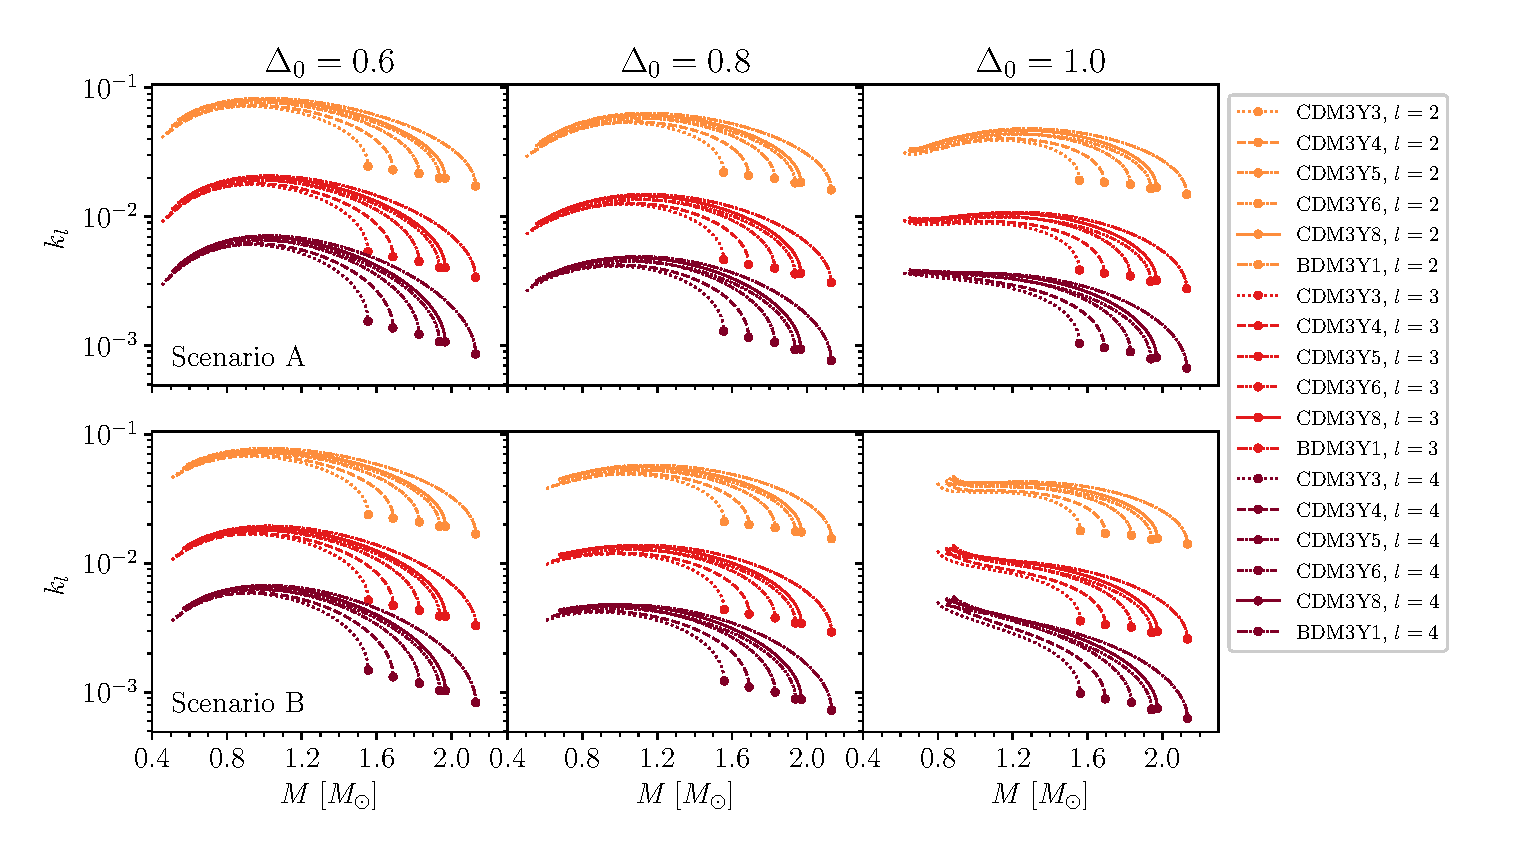
\includegraphics[width=\textwidth]{fig/kl.eps}
        \caption{\gls{GE} tidal Love number at $l$\textsuperscript{th} order $k_l$ as function of \gls{NS} mass computed with 6 density-dependent \gls{NN} interaction versions at different spin polarizations. The dot at the end of each line represents the maximum gravitational mass $M$ of the \gls{NS} generated by the corresponding \gls{EoS}.}
        \label{fig:kl}
\end{figure} 
Alongside with the radii and gravitational mass, the tidal properties of \gls{NS} can also be studied as discussed in Section \ref{sec:gravito_electric_and_gravito_magnetic_tidal_deformation}. The results for \gls{GE} tidal Love number's dependence on \gls{NS}'s gravitational mass arose from 6 versions of the \gls{EoS} are shown in Figure \ref{fig:kl}. Similar to \cite{perot2021role}, in this result, it is clear that the higher the order $l$, the less impactful the Love number $k_l$ is for the tidal properties of the \gls{NS}, i.e. $k_l$ tends to be smaller by an order of magnitude than $k_{l-1}$, as expected from the multipole expansion. The 2\textsuperscript{nd} order is consequently dominant compared to the others. Between two scenarios A and B, at partial polarization of $\Delta_0 = 0.6$, the difference in $k_l$ of the same order is insignificant, except for the small difference in the low mass section. On the other hand, for the case of higher spin polarity in the \gls{NS} surface, the results are much more distinguishable, as the computation with scenario B gives rise to a ``steeper'' curve of $k_l$. Furthermore, in general, the maximum values of $k_l$ are at the common gravitational mass $M$ at all orders computed so far, and this value of $M$ seems to only depends on the value of $\Delta_0$, where the position of maximum $k_l$ tends to be shifted to a higher $M$ as $\Delta_0$ increases. Among these tidal parameters, the only one that has been constrained by far is the dominant 2\textsuperscript{nd} order Love number, which is investigated through the closely related dimensionless tidal deformability parameter of second order $\Lambda_2$ \eqref{eq:Lambda} and whose results are given in Figure \ref{fig:Lambda2}. In the study of \cite{abbott2018gw170817}, the value of $\Lambda_2$ is accepted to be $\Lambda_2 \approx 190^{+390}_{-120}$ at $M=1.4M_\odot$. It is interesting to note that for all cases in this study, this constraint tolerates all \glsplural{EoS} and scenarios, as well as the value of $\Delta_0$, thus no further exclusion can be done with this parameter. It's worth mentioning that the nuclear incompressibility $K$ plays a significant role in determining the tidal deformability $\Lambda_2$ as when $K$ varies from version to version (CDM3Y3 to BDM3Y1), the value of $\Lambda_2$ increases by $\approx 3$ times for the scenario A of $\Delta_0 = 0.6$ case, the same can be said for the different configuration of $\Delta(n_b)$. Testing the values of $k_l$ at higher orders can also be done by evaluating the tidal correction of the \gls{GW} waveform from inspiralling \glsplural{NS} within the PN theory, i.e. the \gls{GE} contribution of order $(2l+1)$PN to the phase of \gls{GW} signal is \citep{perot2021role, yagi2014multipole}
\begin{equation}
    \Psi_l = - \sum^{2}_{i=1} \left[ \frac{5}{16} \frac{(2l-1)!! (4l+3)(l+1)}{(4l-3)(2l-3)} \Lambda_{l,i} X_i^{2l-1} x^{2l - 3/2} + \frac{9}{16} \delta_{l2} \Lambda_{2, i} \frac{X_i^4}{\eta} x^{5/2} \right] + \mathcal{O}(x^{2l-1/2})
\end{equation}
where $i=1,\,2$ is the index distinguishing the two \glsplural{NS} of the system, $x=\left( G\pi Mf/c^3 \right)^{2/3}$, $f$ is the \gls{GW} signal frequency, $M=M_1 + M_2$, $X_i = M_i/M$ and $\eta = M_1 M_2/M^2$.\par
\begin{figure}[ht!]
    \centering
    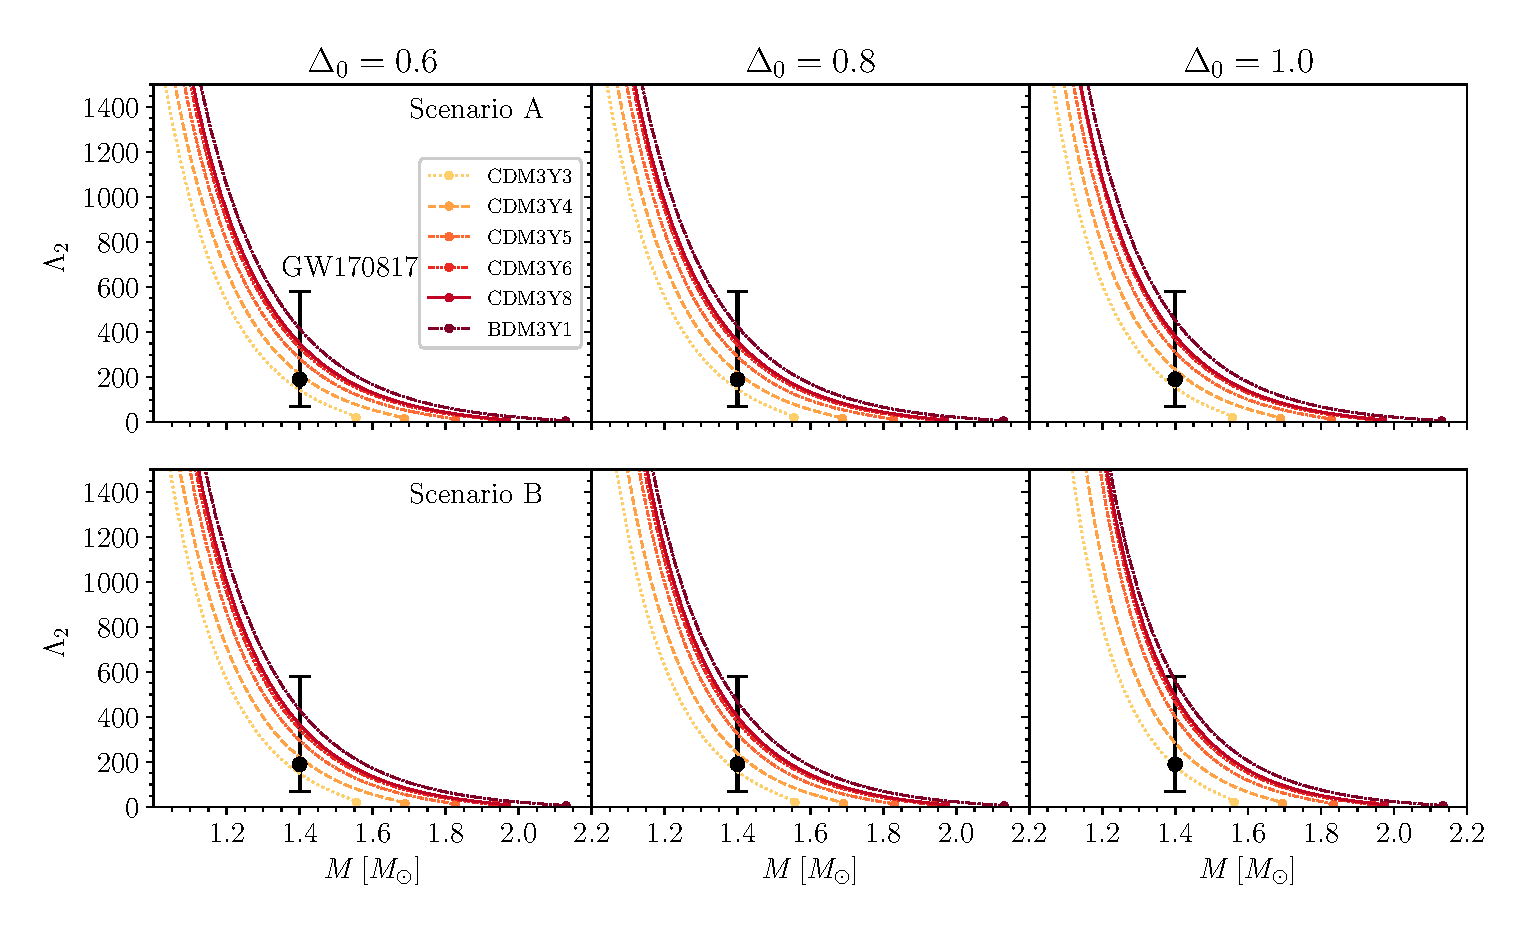
\includegraphics[width=\textwidth]{fig/Lambda2.eps}
    \caption{Dimensionless \gls{GE} tidal deformability parameter of 2\textsuperscript{nd} order $\Lambda_2$ of different CDM3Y$n$ models with varying $\Delta$. The vertical bar is the empirical tidal deformability constraint $\Lambda_2 \approx 190_{-120}^{+390}$ at $1.4M_\odot$, obtained from the Bayesian analysis of GW170817 data with 90\% confidence level \citep{abbott2018gw170817}.}
    \label{fig:Lambda2}
\end{figure} 
The gravito-magnetic tidal Love numbers $j_l$ contribute more weakly to the \gls{GW} phase compared to that of their \gls{GE} counterpart, as the \gls{GM} terms only appear from higher orders of $(2l+2)$PN, where the first correction at 6PN is given by \citep{perot2021role,yagi2017erratum}
\begin{equation}
    \tilde{\Psi}_2 = \sum^{2}_{i=1} \frac{5}{224} \sigma_{2,i} \frac{X_i^4}{\eta} \left( X_i - 1037X_j \right)x^{7/2} + \mathcal{O}(x^{9/2})
\end{equation}
The \gls{GM} tidal Love numbers of second, third and fourth order computed with 6 different \glsplural{EoS} are shown in Figure \ref{fig:jl_stat} for strictly static fluid and \ref{fig:jl_irrot} for irrotational fluid as discussed in Section \ref{sec:gravito_electric_and_gravito_magnetic_tidal_deformation}. Apart from the same trends as the \gls{GE} tidal Love numbers discussed previously, the \gls{GM} Love numbers' values do not have much variation as $\Delta_0$ increases in each scenario, as the shape of each curves in Figure \ref{fig:jl_stat} doesn't differ far from each others except for the difference in range of gravitational mass $M$. The value of $j_l$ corresponding to the \gls{GM} pertubation of irrotational fluid (Figure \ref{fig:jl_irrot}), on the other hand, stands out from the other two types of Love numbers, where its value is completely negative, albeit having the same magnitude as that of static fluid, this type of fluid motion is stated to be more realistic in this case due to it being driven by the tides \citep{perot2021role,pani2018magnetic}. In this case, the lines traced by each interation appear to reach maximum value at the maximum $M$ at the leading terms only, rather than having a local maxima in between. The dominance of the 2\textsuperscript{nd} order terms are clear in all cases, where the difference of around one order of magnitude is remained. Notably, for the \gls{GM} terms corresponding with each \gls{NN} interaction, at higher order $l$, the \gls{NS} mass at maximum $j_l$ seems to become smaller. One more interesting result is that the magnitudes of $j_l$ for two types of fluid are also comparable but is smaller than their \gls{GE} counterpart by one order of magnitude, similar to the conclusion reached by \cite{perot2021role}.
\begin{figure}[ht!]
        \centering
        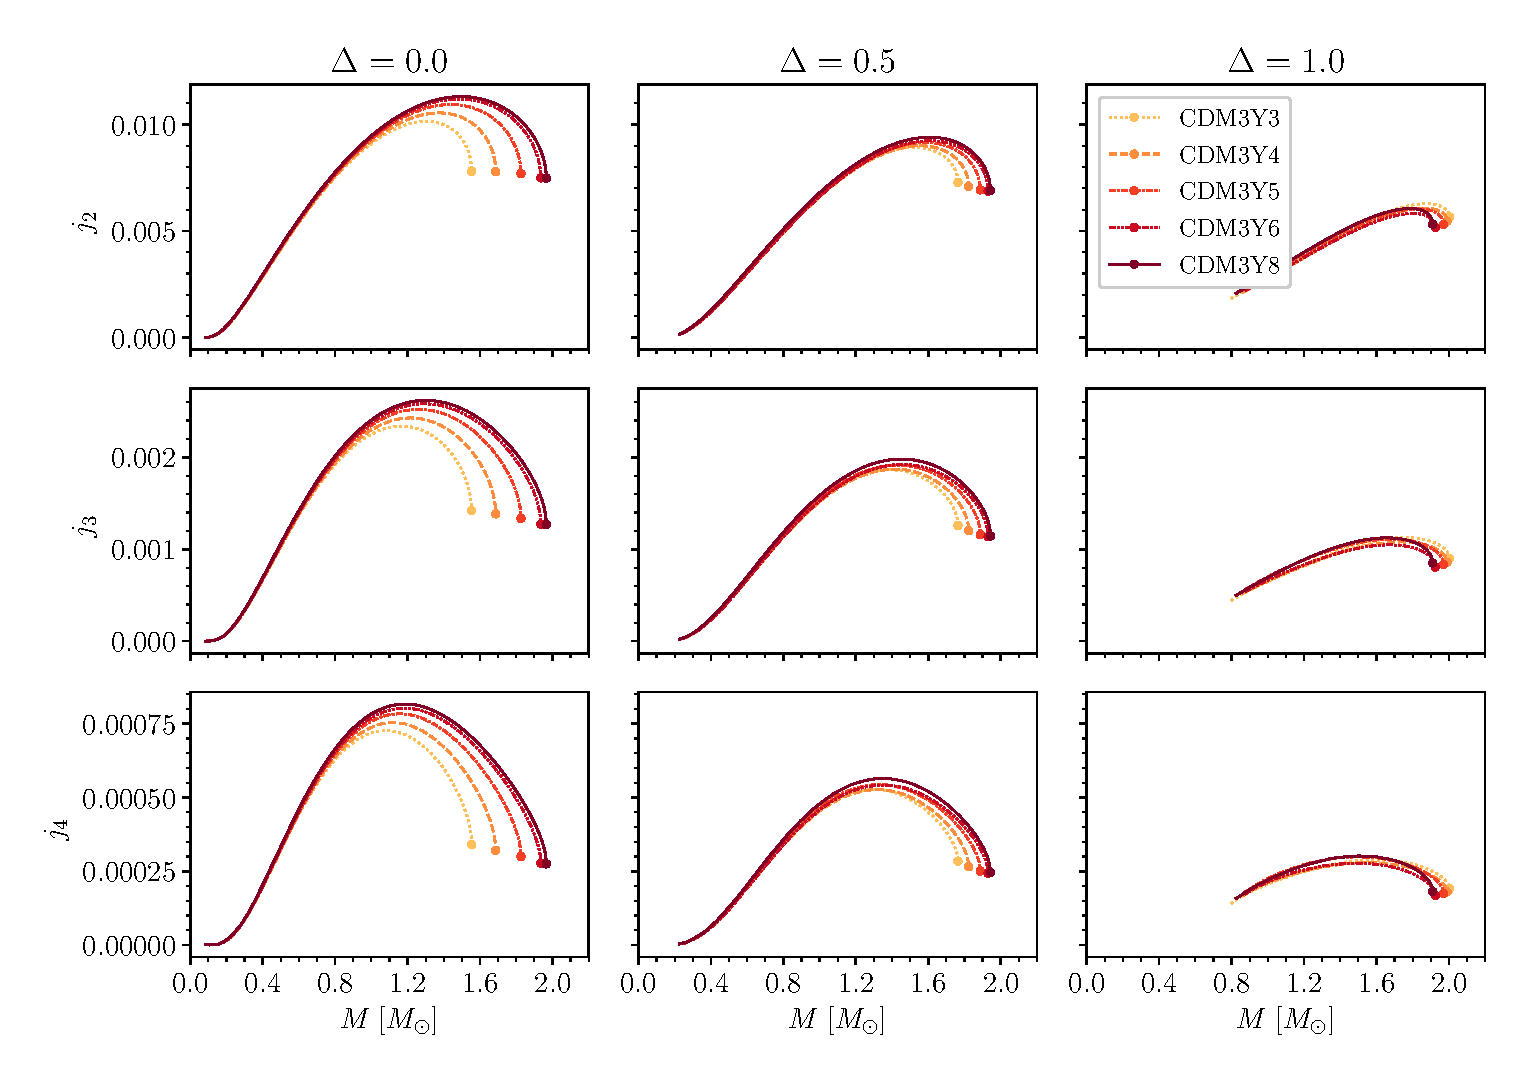
\includegraphics[width=\textwidth]{fig/jl_stat.eps}
        \caption{\gls{GM} tidal Love number at $l$\textsuperscript{nd} order $j_l$ as function of \gls{NS} mass computed with CDM3Y$n$ models of \emph{strictly static fluid} at different polarizations.}
        \label{fig:jl_stat}
\end{figure} 
\begin{figure}[ht!]
        \centering
        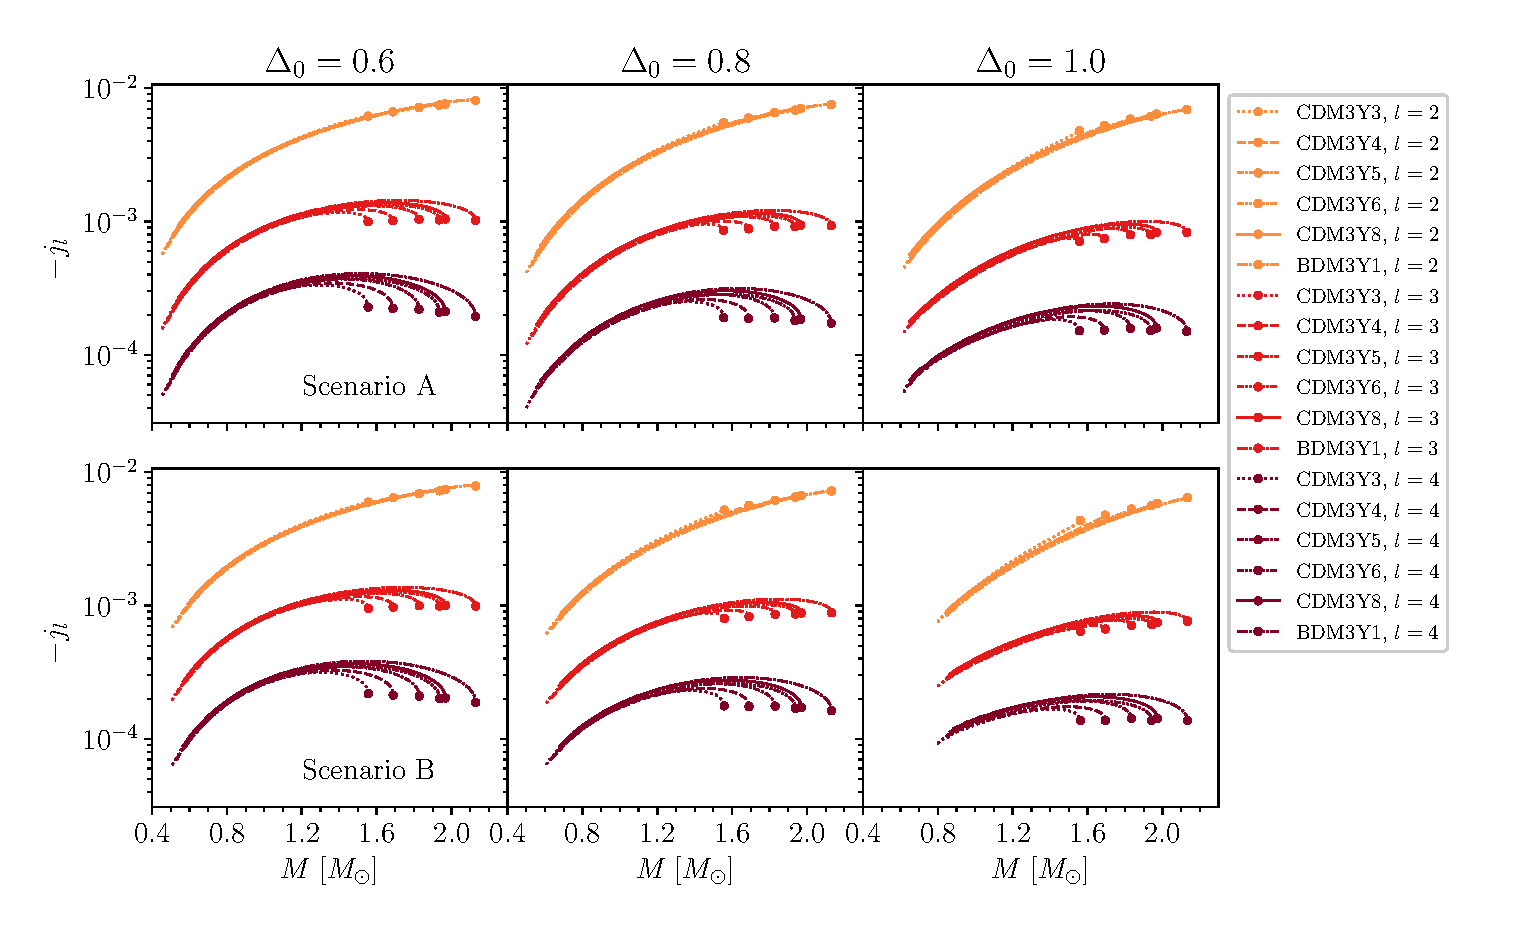
\includegraphics[width=\textwidth]{fig/jl_irrot.eps}
        \caption{\gls{GM} tidal Love number at $l$\textsuperscript{nd} order $j_l$ as function of \gls{NS} mass computed with CDM3Y$n$ models of \emph{irrotational fluid} at different polarizations.}
        \label{fig:jl_irrot}
\end{figure} 
